\documentclass[12pt]{article}

\usepackage{natbib}
\usepackage{url}
\usepackage{siunitx}
\usepackage{graphicx}
\usepackage{grffile}

\graphicspath{{../../Images/Brodatz/}}
\usepackage{subfloat}

\usepackage[T1]{fontenc}
%\usepackage{newpxtext,eulerpx}
\usepackage{txfonts}
\usepackage{microtype}
\usepackage[letterpaper]{geometry}


\title{Research Project\\
Texture Analysis with Information Theory}
\author{Alejandro C.\ Frery
\and Osvaldo A.\ Rosso
\and Eduarda Tatiene Caetano Chagas\footnote{More authors will be included depending on their participation}}
\date{}

\setlength{\parskip}{.1\baselineskip}%

\begin{document}
\maketitle

\section{Introduction}

We intend to apply the ideas presented by \citet{HistoryofArtPaintingsthroughtheLensofEntropyandComplexity2018} to the analysis of SAR textures.
Before this application, we will make an empirical study of the behavior of Information Theory descriptors when applied to the Brodatz textures.
These \num{112} textures \citep[][available at \url{http://sipi.usc.edu/database/database.php?volume=textures}]{TexturesaPhotographicAlbumforArtistsandDesigners1966} have been used as a benchmark for image analysis \citep{TextureFeaturesBasedonTextureSpectrum1991}.
Figure~\ref{fig:13Brodatz} shows thirteen of these textures.

\begin{figure}[hbt]
\centering
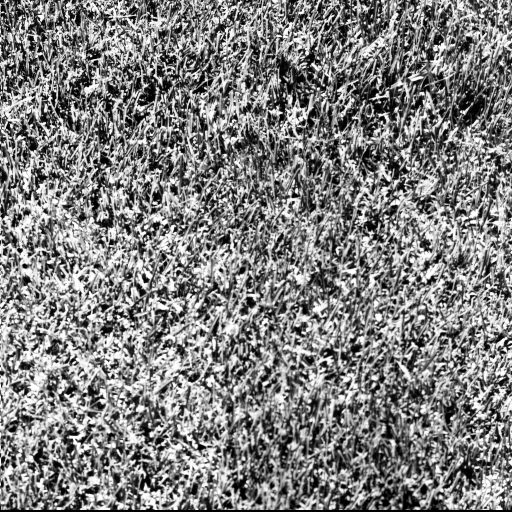
\includegraphics[width=.23\linewidth]{1201png}
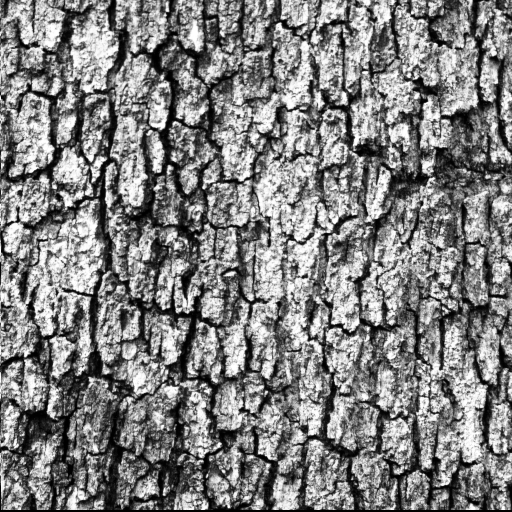
\includegraphics[width=.23\linewidth]{1202png}
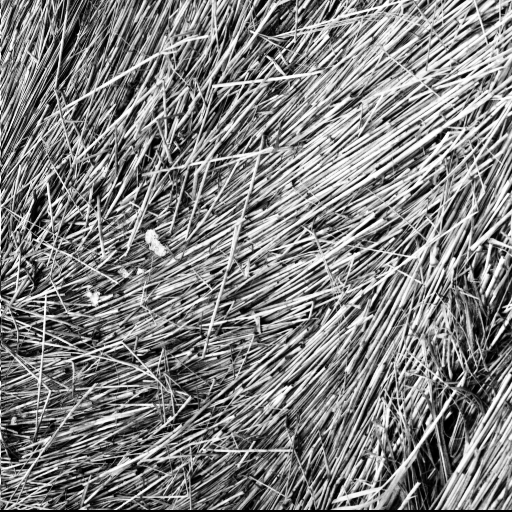
\includegraphics[width=.23\linewidth]{1203png}
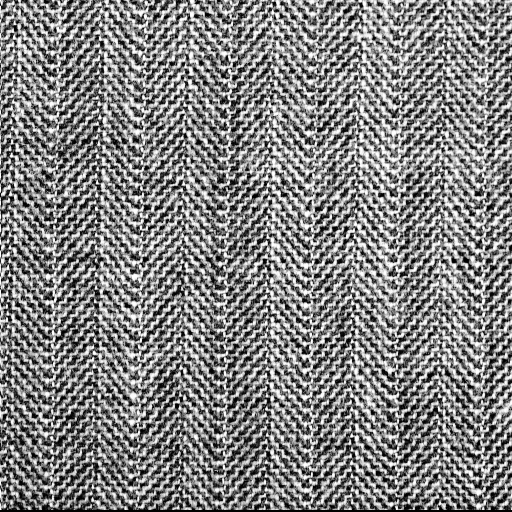
\includegraphics[width=.23\linewidth]{1204png}
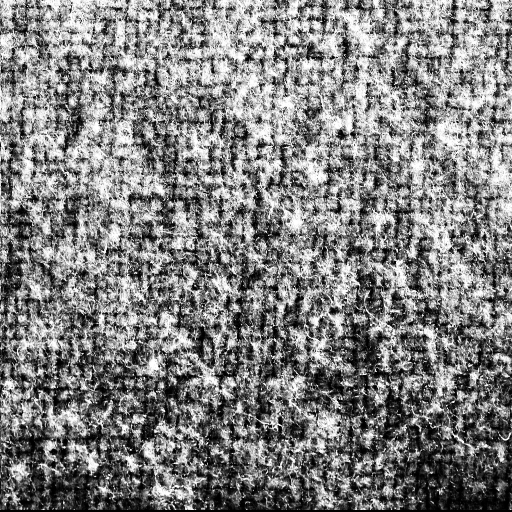
\includegraphics[width=.23\linewidth]{1205png}
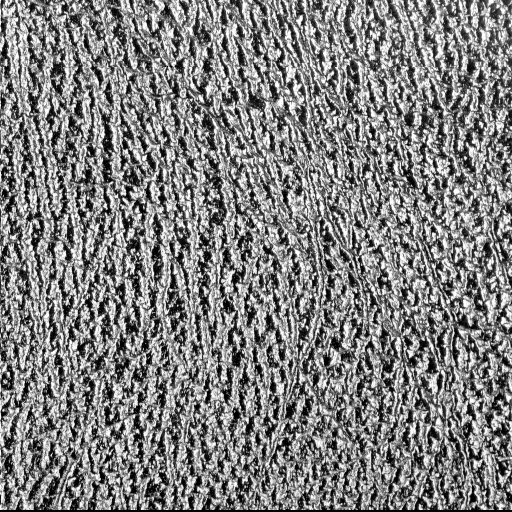
\includegraphics[width=.23\linewidth]{1206png}
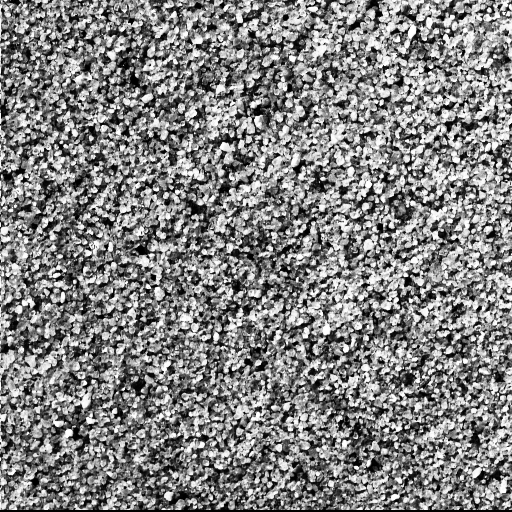
\includegraphics[width=.23\linewidth]{1207png}
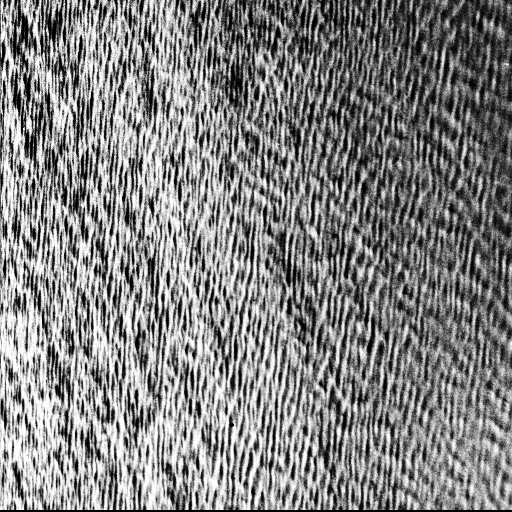
\includegraphics[width=.23\linewidth]{1208png}
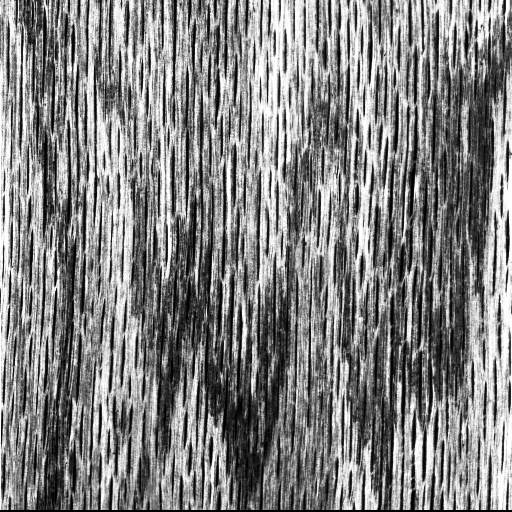
\includegraphics[width=.23\linewidth]{1209png}
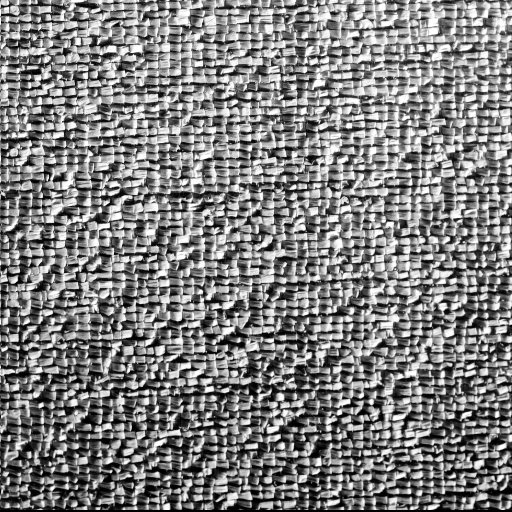
\includegraphics[width=.23\linewidth]{1210png}
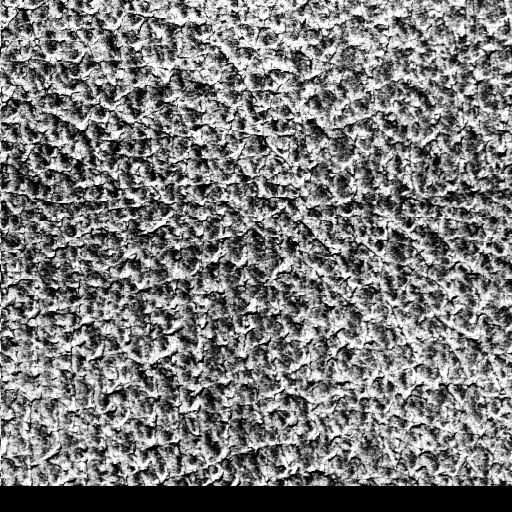
\includegraphics[width=.23\linewidth]{1211png}
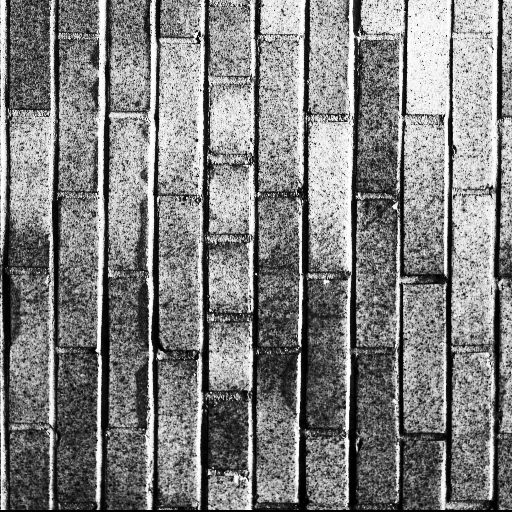
\includegraphics[width=.23\linewidth]{1212png}
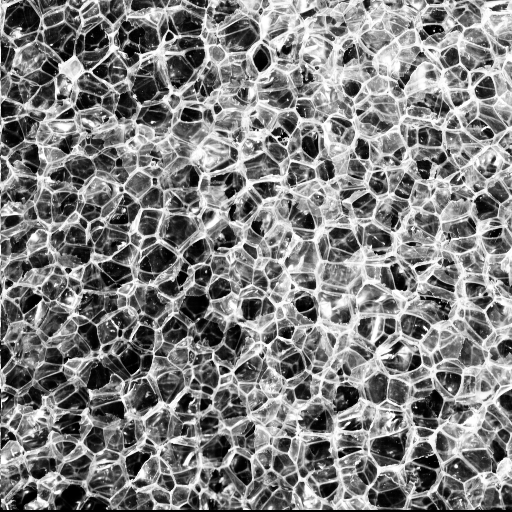
\includegraphics[width=.23\linewidth]{1213png}
\caption{Brodatz textures}\label{fig:13Brodatz}
\end{figure}

\section{Methodology}

{\tiny }We describe here the steps we followed in this research project.

\subsection{Descriptive analysis}

The first step of the study consists in applying the mapping described by \citet{HistoryofArtPaintingsthroughtheLensofEntropyandComplexity2018} to see where the textures are represented in the $\mathcal H\times \mathcal C$ plane.

\subsection{Does contrast impact?}

The second step consists in verifying if contrast impacts on the mapping.
Figure~\ref{fig:TwoTexturesDifferentContrast} shows two of these textures with different contrast.
It is expected that changes in contrast have no effect on the mapping, since the Bandt-Pompe transformation is immune to scalings.

\begin{figure}[hbt]
\centering
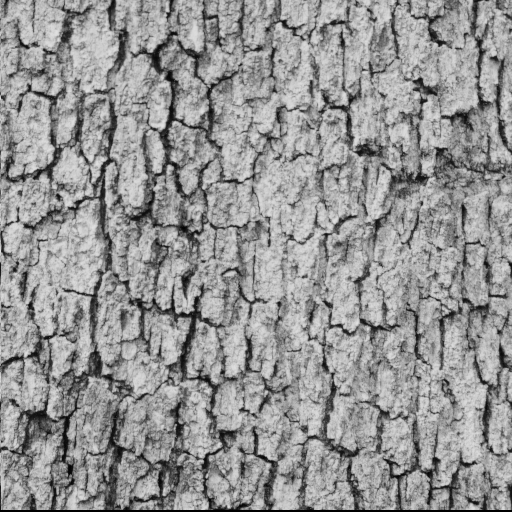
\includegraphics[width=.23\linewidth]{1102png}
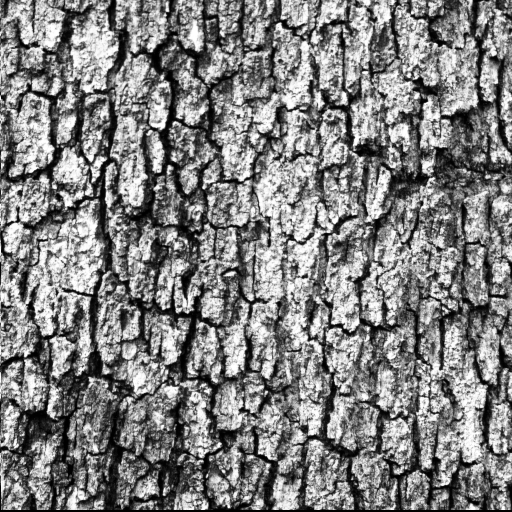
\includegraphics[width=.23\linewidth]{1202png}
\caption{The same texture with different contrast}\label{fig:TwoTexturesDifferentContrast}
\end{figure}

\subsection{Clustering}

The third step consists in verifying if the points in the $\mathcal H\times \mathcal C$ plane form clusters which are \textit{natural} to the eye.

\subsection{Impact of parameters}

The fourth step consists in analyzing the impact that window size and delay have on the mapping of each texture.

\section{First Results}

\subsection{Descriptive analysis}

The first result of study consisted in mapping an set of 45 textures and analysis your behavior, as we can see in Figure~\ref{fig:textureshC}.

\begin{figure}[!h]
	\centering
	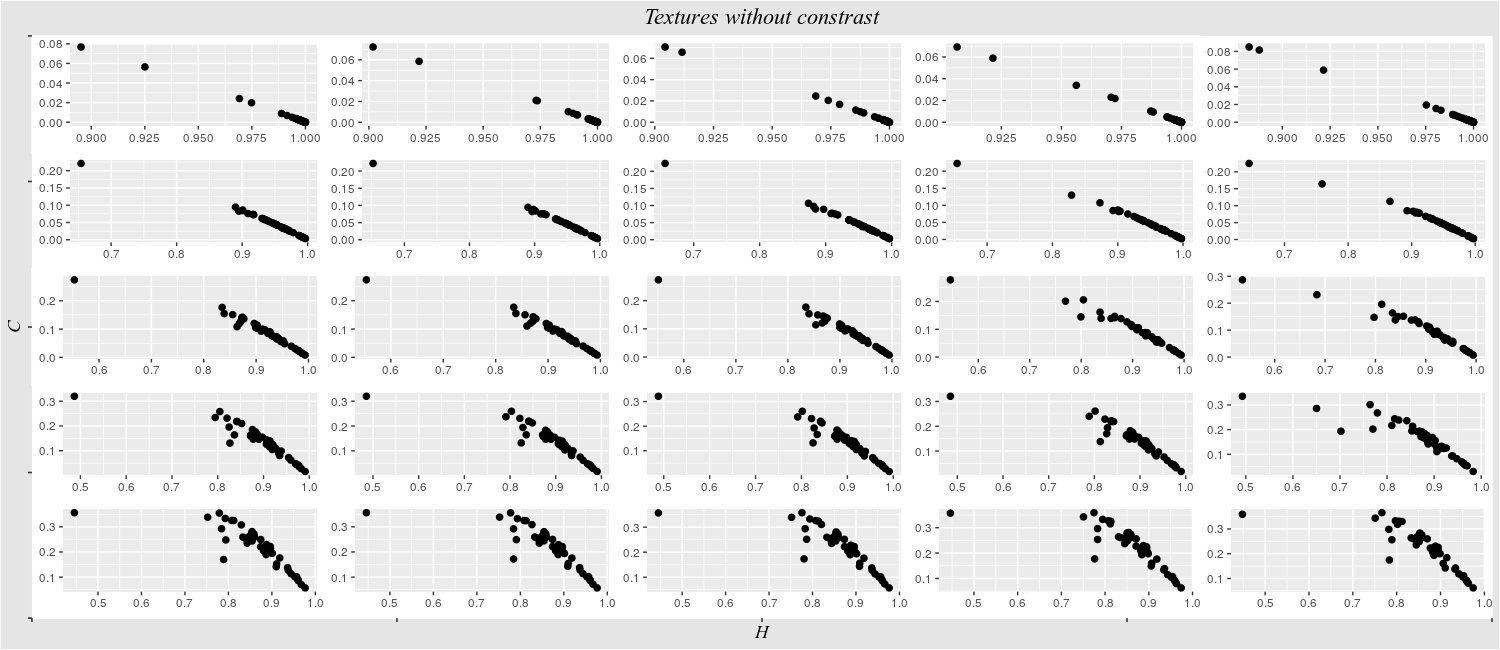
\includegraphics[scale = 0.42]{../../Images/Textures/Textures_no_contrast.png}        
	\caption{Set of Brodatz textures mapping in $\mathcal H\times \mathcal C$ plane}
	\label{fig:textureshC}
\end{figure}


\subsection{Does contrast impact?}

For analyze the impact of the contrast in the mapping in the $\mathcal H\times \mathcal C$ plane, we separate two sets of textures, one with contrast apply and another not. The result we can see in Figure~\ref{fig:texturescontrastHC}, where the colors represent the different textures and the shape inform the apply or not of contrast (triangles represents textures without contrast).

\begin{figure}[!h]
	\centering
	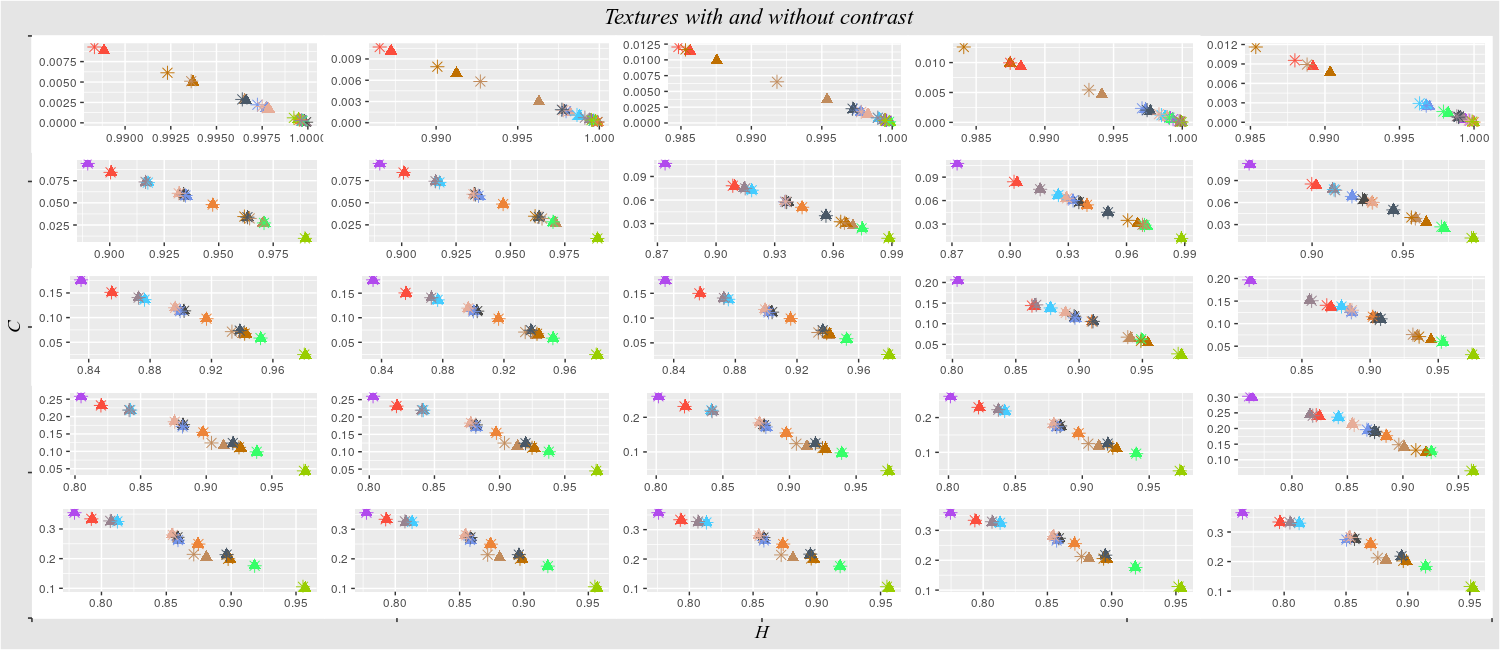
\includegraphics[scale = 0.42]{../../Images/Textures/Textures_Contrast.png}        
	\caption{Set of Brodatz textures with and without contrast mapping in $\mathcal H\times \mathcal C$ plane}
	\label{fig:texturescontrastHC}
\end{figure}

\subsection{Clustering and Impact of parameters}

We can observe that the settings of the Plane $ (D = 5, \tau = 1) $, $ (D = 5, \tau = 2) $, $ (D = 5, \tau = 4) $ can divide the set of textures into three subgroups, as shown in Figure~\ref{fig:clusters}. However, the impact of the contrast makes no difference in the plane view, although the characterization of the textures in Figure~\ref{fig:texturescontrastHC} was perfectly done in the plane by applying the settings $ (D = 3, \tau = 5) $ .

\begin{figure}[!h]
	\centering
	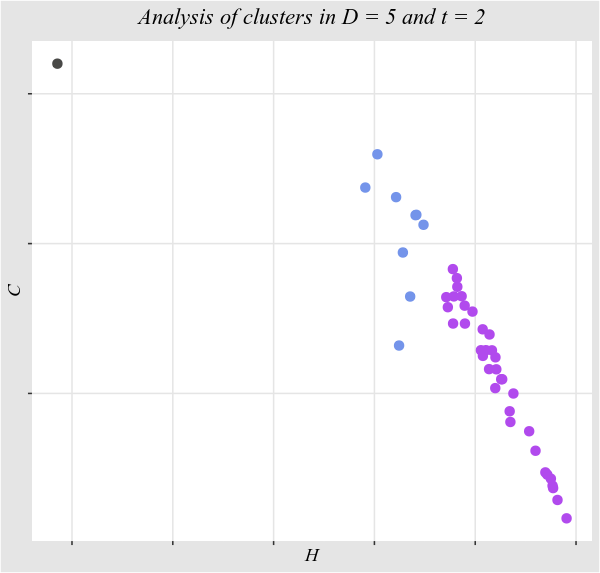
\includegraphics[scale = 0.6]{../../Images/Textures/cluters_textures.png}        
	\caption{Clusters formed after the mapping in the $\mathcal H\times \mathcal C$ plane}
	\label{fig:clusters}
\end{figure}

\bibliographystyle{agsm}
\bibliography{../../Common/references}
\end{document}